\documentclass[conference]{IEEEtran}
\IEEEoverridecommandlockouts
% Template version as of 6/27/2024 (IEEE). Full working draft.

\usepackage{cite}
\usepackage{amsmath,amssymb,amsfonts}
\usepackage{amsthm}
\usepackage{algorithm}
\usepackage{algorithmic}
\usepackage{graphicx}
\usepackage{booktabs}
\usepackage{multirow}
\usepackage{textcomp}
\usepackage{xcolor}
\usepackage{bm}

\graphicspath{{figures/}}

\def\BibTeX{{\rm B\kern-.05em{\sc i\kern-.025em b}\kern-.08em
    T\kern-.1667em\lower.7ex\hbox{E}\kern-.125emX}}

% ---- Theorem environments ----
\newtheorem{theorem}{Theorem}
\newtheorem{lemma}{Lemma}
\newtheorem{proposition}{Proposition}
\newtheorem{corollary}{Corollary}
\theoremstyle{definition}
\newtheorem{definition}{Definition}
\newtheorem{assumption}{Assumption}
\theoremstyle{remark}
\newtheorem{remark}{Remark}

% ---- Notation macros ----
\newcommand{\Slots}{T}
\newcommand{\Ep}{L}
\newcommand{\Neps}{K}
\newcommand{\Ntn}{N}
\newcommand{\rhobind}{\rho}
\newcommand{\load}{\eta}
\newcommand{\type}{\theta}
\newcommand{\typesp}{\Theta}
\newcommand{\alloc}{x}
\newcommand{\allocsp}{\mathcal{X}}
\newcommand{\wt}{w}
\newcommand{\val}{v}
\newcommand{\flo}{f}
\newcommand{\bindind}{b}
\newcommand{\Reg}{\mathrm{Reg}}
\newcommand{\Slack}{\Delta}
\newcommand{\Otil}{\tilde{O}}
\newcommand{\E}{\mathbb{E}}
\newcommand{\R}{\mathbb{R}}
\newcommand{\ind}{\mathbb{1}}
\newcommand{\Wel}{\mathcal{W}}

\begin{document}

\title{The Incentive--Learning Frontier: Truthful Reinforcement-Learning PRB Allocation Under Hard Service Floors in O-RAN Slicing}

\author{\IEEEauthorblockN{Prashant Mishra}
\IEEEauthorblockA{\textit{G. S. Sanyal School of Telecommunications} \\
\textit{Indian Institute of Technology Kharagpur}\\
Kharagpur, India}
\and
\IEEEauthorblockN{Dibbendu Roy}
\IEEEauthorblockA{\textit{G. S. Sanyal School of Telecommunications} \\
\textit{Indian Institute of Technology Kharagpur}\\
Kharagpur, India}
}

\maketitle

\begin{abstract}
Open RAN increasingly delegates slice-level physical resource block (PRB) allocation to learning agents in the near-real-time RIC, yet these agents assume the controller observes tenant demand directly. We study the setting in which tenants are strategic and the allocator learns from their reports, so that each report is simultaneously an incentive object and a training sample. We show that exact dominant-strategy truthfulness within a fixed-policy epoch coexists with an unavoidable episode-level incentive slack whenever hard per-slice service floors are active, and we localize that slack precisely to the slots on which a floor binds. Our main result characterizes the achievable tradeoff between cumulative learning regret and incentive slack as a frontier governed by two parameters, the epoch length $\Ep$ and the service-floor binding frequency $\rhobind$, and proves that $\rhobind$ is an exogenous quantity fixed by admission-control load rather than by the learning horizon. The combined cost is of order $\rhobind^{1/3}\Slots^{2/3}$, which recovers the known single-lever barrier when floors always bind and is strictly smaller otherwise. We instantiate the frontier on the ns-3 5G-LENA simulator through a plain-socket bridge that couples a Python RL+DSIC controller to a 3GPP-compliant PHY/MAC, and we show experimentally that (i) the measured binding frequency is set by load and is flat in $\Ep$, (ii) the measured incentive slack is null exactly where $\rhobind\to0$, and (iii) the truthful learned allocator matches round-robin, max-CQI and proportional-fair scheduling on throughput and, among floor-guaranteeing policies under overload, is best on every QoS-and-efficiency axis at once---lowest URLLC tail latency, best priority-weighted SLA, lowest aggregate SLA, and fewest wasted PRBs---while uniquely guaranteeing service floors. A strategic-reporting study confirms the mechanism is dominant-strategy truthful---the tenant's best response is exactly truthful and the same allocator with the payment removed is gamed for a double-digit utility gain that starves the honest slices---so the Myerson payment, not the allocation rule, is what makes a demand-responsive learner strategy-proof.
\end{abstract}

\begin{IEEEkeywords}
O-RAN, network slicing, mechanism design, incentive compatibility, reinforcement learning, resource allocation, regret.
\end{IEEEkeywords}

\section{Introduction}\label{sec:intro}
Open RAN (O-RAN) decomposes the radio access network into interoperable components and exposes radio resource control to applications hosted in the near-real-time RAN Intelligent Controller (RIC)~\cite{ref:oran}. Within this architecture, slice-level allocation of physical resource blocks (PRBs) is increasingly delegated to reinforcement-learning (RL) agents that observe radio and traffic key performance measurements and emit an allocation once per control interval. A growing body of work demonstrates such RL xApps for PRB and slice management~\cite{ref:coloran,ref:slicing}.

This literature shares an assumption that is rarely made explicit: the controller observes tenant demand. The measurements that drive allocation (buffer occupancy, PRB utilization, throughput, delay) are taken as ground truth about how much each slice needs. In a multi-tenant deployment, however, slices belong to distinct self-interested tenants, and the only interface between a tenant and the controller is a report. Once the controller \emph{learns} its policy from these reports, each report plays two roles at once: it is the object on which incentives act, since a tenant may benefit from overstating need, and it is a training sample that shapes the policy applied in the future. To our knowledge, the interaction between strategic reporting and policy learning is absent from the O-RAN slicing literature.

This coupling creates a tension that single-round mechanism design does not resolve. One can make the per-interval allocation truthful: a monotone allocation rule with the appropriate payment is dominant-strategy incentive compatible (DSIC)~\cite{ref:myerson}. But a learning policy whose parameters depend on the history of reports can be manipulated \emph{across} intervals, because a tenant who misreports early can steer the policy toward configurations that favor it later, even when each interval in isolation is truthful~\cite{ref:huh}. The natural question is quantitative: what is the exact exchange rate between how fast the controller learns and how much episode-level truthfulness it must surrender, and is that exchange rate governed by a quantity the operator can measure?

We answer this for the constrained setting O-RAN imposes, in which each slice carries a hard service floor, a minimum guaranteed allocation. Our contributions are:
\begin{itemize}
\item \textbf{Within-epoch exact DSIC} for an epoch-frozen learning allocator with a monotone inner allocation rule (Theorem~\ref{thm:dsic}).
\item A \textbf{constrained dynamic-IC impossibility}, with the obstruction \emph{localized} to the slots on which a service floor binds, and identically zero when no floor binds (Theorem~\ref{thm:imposs}).
\item The \textbf{incentive--learning frontier}: learning regret $\Otil(\sqrt{\Ep\Slots})$ and manipulation slack $O(\rhobind\Slots/\Ep)$ are achieved simultaneously, and their balance over the epoch length gives combined cost $\Otil(\rhobind^{1/3}\Slots^{2/3})$ (Theorem~\ref{thm:frontier}).
\item A \textbf{binding-frequency invariance lemma}: $\rhobind$ is fixed by admission-control load and is asymptotically independent of the epoch length, which is what makes it a second, freely tunable axis (Lemma~\ref{lem:invariance}).
\item A \textbf{reproducible instantiation}: an epoch-frozen DSIC-RL allocator (Section~\ref{sec:algo}), a plain-socket Python$\leftrightarrow$ns-3 5G-LENA bridge that carries per-slice PRB budgets and returns 3GPP-measured KPIs (Section~\ref{sec:impl}), and an evaluation (Section~\ref{sec:eval}) that validates all three predictions and compares the truthful learned allocator against classical schedulers.
\item A \textbf{strategy-proofness study} that measures the best-response manipulation gain of every scheduler and, via a payment-ablated version of our own allocator, isolates the Myerson payment as the lever that makes a demand-responsive learner truthful without discarding the demand signal (Section~\ref{sub:robust}).
\end{itemize}

The distinguishing feature of our characterization is its second lever. Prior analyses of learning under truthfulness expose a single knob, the update granularity, and a single barrier: freezing the policy for longer suppresses manipulation but slows learning, yielding a worst-case combined cost of order $\Slots^{2/3}$~\cite{ref:dai,ref:dekel}. We show that under hard floors the manipulation cost is not a function of update granularity alone; it is gated by how often a floor binds, and that frequency is exogenous, set by admission-control load rather than by the learning horizon. The achievable region is therefore a surface in two parameters, and in the underloaded regime O-RAN targets it lies strictly inside the single-lever barrier---a claim we confirm empirically, where the floor-always-active ($\rhobind\!=\!1$) baseline is measurably worse than our load-gated allocator.

\textbf{Relation to closest prior art.} Dai, Golrezaei and Jaillet~\cite{ref:dai} independently propose epoch-based lazy updates for incentive-aware allocation under long-term cost constraints, attaining $\Otil(\sqrt{\Slots})$ welfare regret with a near-truthful equilibrium; their model is an abstract single-resource setting with no networking content, their learner is primal-dual rather than RL, and their guarantee is approximate truthfulness in equilibrium rather than exact within-epoch dominance. Huh and Kandasamy~\cite{ref:huh} establish that single-round IC need not imply truthfulness across rounds against non-myopic agents. We retain exact within-epoch DSIC with a learned allocator, localize the residual obstruction to the active-constraint wedge, and parametrize the resulting frontier by a measurable physical quantity, instantiated in a 3GPP-compliant RAN simulator.

\section{Related Work}\label{sec:related}
\textbf{Dynamic mechanism design and learning.} The dynamic pivot~\cite{ref:bergemann} and virtual-pivot~\cite{ref:kakade} mechanisms achieve periodic ex-post incentive compatibility for efficient and revenue-optimal dynamic allocation respectively. A recent line learns such mechanisms online, recovering dynamic VCG with welfare and truthfulness regret. Closest to us, \cite{ref:dai} freezes dual variables within epochs to suppress manipulation, hitting $\Otil(\sqrt{\Slots})$ welfare regret with a one-directional $\Omega(\Slots^{2/3})$ learning barrier under switching costs~\cite{ref:dekel}. We differ in three ways: we keep \emph{exact} within-epoch DSIC under a deep-RL allocator, we expose a \emph{second} lever (binding frequency), and we instantiate the result in a RAN system.

\textbf{Auctions and incentives for slicing.} Truthful, mostly static, VCG-style auctions exist for RAN, spectrum, and slice allocation, and network-slicing games model tenants as strategic via share-constrained allocation~\cite{ref:slicinggames}. None couples a hard-floor-constrained \emph{learning} allocator with truthfulness guarantees.

\textbf{RL for O-RAN slicing.} DRL and constrained multi-agent RL drive PRB and slice control in the RIC~\cite{ref:coloran,ref:slicing}, including safe-RL formulations enforcing SLA constraints. Across this literature the controller is assumed to observe true demand; tenants are never modeled as strategic agents with private types whose reports also train the allocator.

\textbf{Classical MAC scheduling.} Round-robin, max-CQI/max-rate, and proportional-fair (PF) schedulers~\cite{ref:pf} are the reference points for 5G MAC resource assignment and span the fairness--throughput axis. They assume observed demand and carry no incentive guarantee; we use them as performance baselines in Section~\ref{sec:eval}.

\section{System Model}\label{sec:model}
Fig.~\ref{fig:arch} shows the setting: a strategic-reporting layer feeds an epoch-frozen learned allocator in the near-RT RIC, whose per-slice PRB budget is enforced on a 3GPP PHY/MAC and whose measured KPIs close the RL loop.

\begin{figure}[t]
\centering
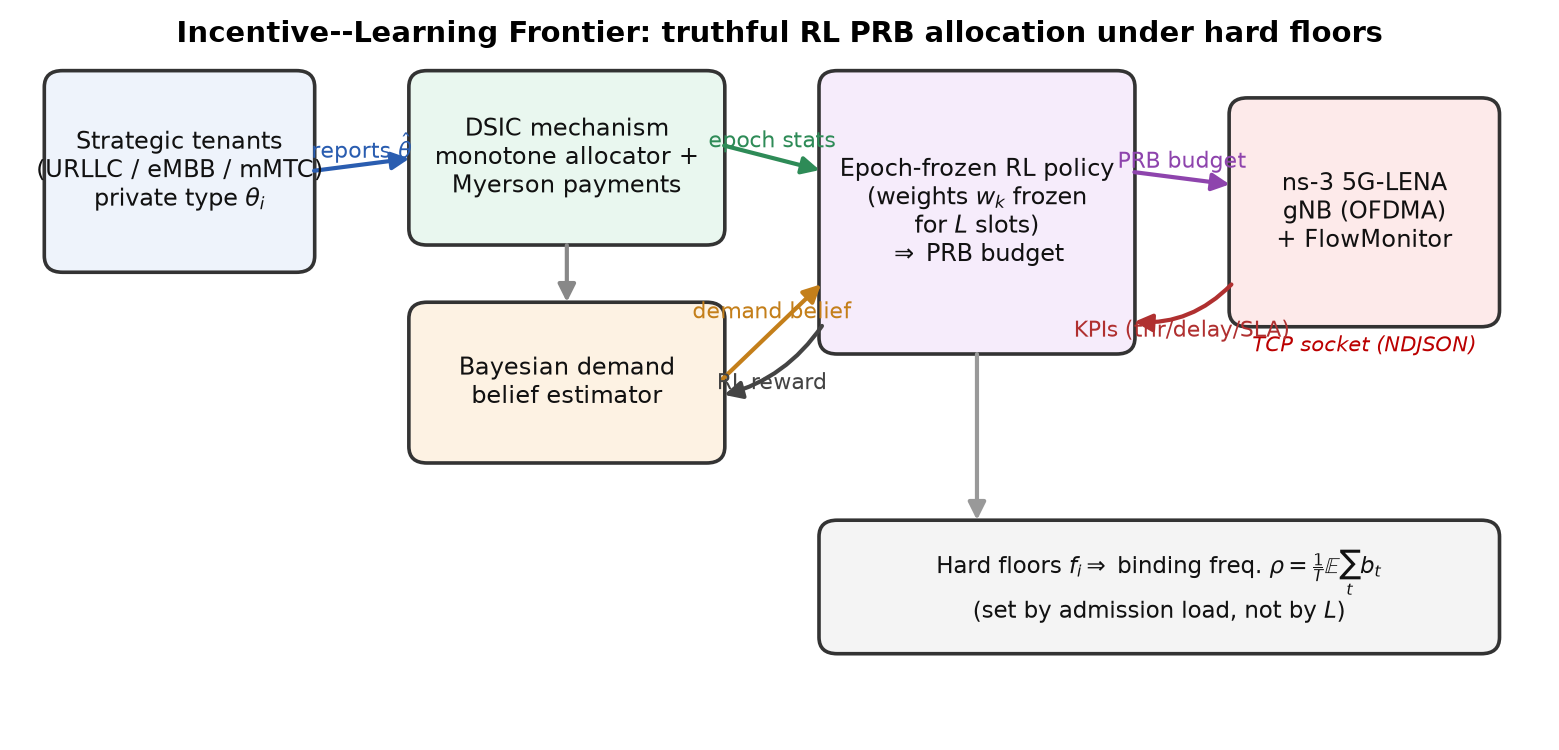
\includegraphics[width=0.98\columnwidth]{architecture.png}
\caption{GTMD-RL architecture and its 5G-LENA instantiation. Tenants submit demand reports; the RIC runs a Bayesian demand belief and an epoch-frozen RL policy that emits per-slice weights; a monotone weighted-greedy inner allocator turns weights into a PRB budget with Myerson payments. The budget is shipped over a TCP socket to the ns-3 5G-LENA gNB, which enforces it, runs the epoch on a 3GPP-compliant PHY/MAC, and returns per-slice throughput/delay as the RL reward.}
\label{fig:arch}
\end{figure}

\subsection{Slots, epochs, tenants}
Time is slotted, $t\in\{1,\dots,\Slots\}$, partitioned into $\Neps=\Slots/\Ep$ epochs of length $\Ep$. A set $[\Ntn]$ of tenants (slices) shares a cell of $B$ PRBs. Tenant $i$ holds a private scalar demand-intensity type $\type_i\in\typesp=[\underline{\type},\bar{\type}]$, drawn i.i.d.\ within an epoch from an epoch-stationary law (Assumption~\ref{ass:stat}).

\subsection{Reports, allocation, valuations}
At the start of epoch $k$ the mechanism fixes a weight vector $\wt_k\in\R_{\ge0}^{\Ntn}$, the output of the RL policy, held constant across the epoch. Each tenant submits a report $\hat\type_i$. Given $(\hat\type,\wt_k)$, a per-slot inner allocator returns a feasible split $\alloc_t\in\allocsp=\{\alloc\in\R_{\ge0}^{\Ntn}:\sum_i\alloc_i\le B\}$, with $g_i(\hat\type_i;\wt_k)$ the per-slot share assigned to $i$. Tenant $i$ derives per-slot value $\val_i(\alloc_{i,t};\type_i)$ and has quasi-linear utility $\val_i-p_i$ for payment $p_i$.

\begin{assumption}[Single crossing]\label{ass:sc}
$\val_i(\cdot;\cdot)$ is concave and increasing in the allocation and satisfies the Spence--Mirrlees condition $\partial^2\val_i/\partial\alloc_i\,\partial\type_i\ge0$.
\end{assumption}

\subsection{Service floors and the binding indicator}
A subset of slots imposes a hard floor $\alloc_{i,t}\ge\flo_i$ for constrained tenants. Define the per-slot binding indicator
\begin{equation}
\bindind_t=\ind[\text{a floor is active and allocation-limited at slot }t],
\end{equation}
and the binding frequency $\rhobind=\tfrac{1}{\Slots}\,\E\sum_{t=1}^{\Slots}\bindind_t\in[0,1]$. Here ``allocation-limited'' means the floor, rather than the tenant's own demand, is the active constraint determining $\alloc_{i,t}$.

\subsection{Epoch-frozen mechanism, learning, and payments}
The weight $\wt_k$ depends only on data observed in epochs $<k$; the between-epoch update is any no-regret learner applied to per-epoch aggregate statistics. Two consequences are used throughout. First, within an epoch the allocation rule is a fixed function of reports. Second, because $\wt_{k+1}$ is computed from the empirical statistics of the $\Ep$ slots of epoch $k$, any single tenant's marginal influence on $\wt_{k+1}$ is diluted by the epoch size.

\begin{assumption}[Monotone inner allocator]\label{ass:mono}
For fixed $\wt_k$, $g_i(\hat\type_i;\wt_k)$ is nondecreasing in $\hat\type_i$, pointwise per slot, and continuous in $\wt_k$, with ties broken to preserve continuity.
\end{assumption}

\begin{assumption}[Bounded marginal influence]\label{ass:infl}
The between-epoch map satisfies $\lVert\partial\wt_{k+1}/\partial\hat\type_{i,k}\rVert=O(1/\Ep)$, where $\hat\type_{i,k}$ is tenant $i$'s report in epoch $k$.
\end{assumption}

\begin{assumption}[Epoch stationarity and exogenous load]\label{ass:stat}
Within each epoch the arrival process is stationary and ergodic, and the offered load factor $\load<1$ is set by admission control, not by the learned weights $\wt_k$.
\end{assumption}

Payments use the Myerson critical value of the frozen per-epoch allocation rule:
\begin{equation}\label{eq:payment}
p_i(\hat\type_i)=\hat\type_i\,a_i(\hat\type_i)-\int_{\underline{\type}}^{\hat\type_i} a_i(z)\,dz,
\end{equation}
where $a_i(\hat\type_i)=\sum_{t\in\text{epoch}}g_i(\hat\type_i;\wt_k)$ is the epoch-aggregate allocation to $i$.

\section{Within-Epoch Truthfulness}\label{sec:dsic}

\begin{theorem}[Within-epoch exact DSIC]\label{thm:dsic}
Under Assumptions~\ref{ass:sc} and \ref{ass:mono}, with payments \eqref{eq:payment}, truthful reporting is a dominant strategy for every tenant within each epoch.
\end{theorem}

\begin{proof}
Fix epoch $k$. By construction $\wt_k$ is independent of the reports submitted in epoch $k$, so within the epoch the environment is a static single-parameter mechanism with allocation rule $a_i(\cdot)$ and payment \eqref{eq:payment}. Assumption~\ref{ass:mono} makes each per-slot rule $g_i(\cdot;\wt_k)$ nondecreasing in $\hat\type_i$, and a sum of nondecreasing functions is nondecreasing, so $a_i$ is monotone. Under the Spence--Mirrlees condition (Assumption~\ref{ass:sc}), monotonicity of the allocation together with the threshold payment \eqref{eq:payment} is necessary and sufficient for dominant-strategy truthfulness in a single-parameter domain~\cite{ref:myerson}. Payments and values are additive across the slots of the epoch and $\wt_k$ is fixed, so the per-slot guarantees aggregate to the epoch. Hence truthful reporting maximizes $\val_i(a_i(\hat\type_i);\type_i)-p_i(\hat\type_i)$ for every $\type_{-i}$.
\end{proof}

\begin{remark}
Theorem~\ref{thm:dsic} lets the remainder of the paper speak only of \emph{cross}-epoch slack: within an epoch there is none. The single load-bearing requirement is pointwise monotonicity of the inner allocator (Assumption~\ref{ass:mono}), which the weighted-greedy allocator of Section~\ref{sec:algo} satisfies by construction; we verify this numerically over $200$ random report perturbations.
\end{remark}

\section{The Cost of Learning Under Hard Floors}\label{sec:imposs}

We now show that the only way to game the mechanism is across epochs, and that the resulting slack lives entirely on binding slots.

\begin{theorem}[Localized dynamic-IC impossibility]\label{thm:imposs}
Suppose the between-epoch update is nontrivial, i.e.\ $\partial\wt_{k+1}/\partial\hat\type_{i,k}\neq0$. If $\rhobind>0$ the mechanism is not exactly dynamic-IC across the episode. Moreover the per-tenant dynamic-IC slack satisfies
\begin{equation}\label{eq:slacklocal}
\Slack_i=\Theta\!\Big(\E\sum_{t}\bindind_t\,\mu_{i,t}\Big),
\end{equation}
where $\mu_{i,t}$ is the shadow price of the floor at slot $t$; the slack is supported on binding slots, and $\Slack_i=0$ whenever $\rhobind=0$.
\end{theorem}

\begin{proof}[Proof sketch]
By Theorem~\ref{thm:dsic} no within-epoch deviation is profitable, so the only manipulation channel is the effect of a current report on future weights. Consider a one-shot deviation by tenant $i$ in epoch $k$ and decompose its first-order effect on $i$'s future utility into a component aligned with the welfare objective the learner ascends and a residual ``wedge''. On non-binding slots the realized allocation is interior, the per-epoch program is locally smooth, and the envelope theorem cancels the welfare-aligned component: at an interior constrained optimum, marginal values are equalized up to the budget multiplier and the tenant's wedge vanishes. On binding slots the floor is active, the allocation sits at a kink, and the envelope identity fails, leaving a residual equal to the floor's shadow price $\mu_{i,t}$. Summing gives \eqref{eq:slacklocal}; with $\rhobind=0$ there are no binding slots and the residual is identically zero. The full argument, including the differentiability conditions supplied by Assumption~\ref{ass:mono}, is in Appendix~\ref{app:imposs}.
\end{proof}

\begin{remark}[Distinction from constrained-efficiency impossibility]
Classical results assert that constrained-efficient mechanisms are not incentive compatible. Theorem~\ref{thm:imposs} instead \emph{localizes} the obstruction to the active-constraint wedge and shows it is null when floors never bind. This localization, not the bare impossibility, is what enables the two-parameter frontier below.
\end{remark}

\section{The Incentive--Learning Frontier}\label{sec:frontier}

\begin{theorem}[Two-parameter frontier]\label{thm:frontier}
The epoch-frozen mechanism satisfies simultaneously
\begin{align}
\Reg(\Slots)&=\Otil\!\big(\sqrt{\Ep\,\Slots}\big),\label{eq:reg}\\
\Slack(\Slots)&=O\!\big(\rhobind\,\Slots/\Ep\big),\label{eq:slack}
\end{align}
and, within the class of epoch-frozen mechanisms with a monotone inner allocator, these are jointly tight up to logarithmic factors. Balancing \eqref{eq:reg} and \eqref{eq:slack} over the epoch length yields the optimum
\begin{equation}\label{eq:opt}
\Ep^\star=\Theta\!\big(\rhobind^{2/3}\Slots^{1/3}\big),\qquad
\Reg+\Slack=\Otil\!\big(\rhobind^{1/3}\Slots^{2/3}\big).
\end{equation}
At $\rhobind=1$ this recovers the $\Slots^{2/3}$ barrier; for $\rhobind<1$ it is strictly smaller by a factor $\rhobind^{1/3}$.
\end{theorem}

\begin{proof}[Proof sketch]
\emph{Regret \eqref{eq:reg}.} The policy changes only $\Neps=\Slots/\Ep$ times. Treating each epoch as one round of a no-regret learner whose per-round loss ranges over $[0,\Ep]$, online gradient descent attains meta-regret $\Otil(\Ep\sqrt{\Neps})=\Otil(\sqrt{\Ep\,\Slots})$ in cumulative slot units.
\emph{Slack \eqref{eq:slack}.} A manipulation in epoch $k$ perturbs $\wt_{k+1}$ by $O(1/\Ep)$ (Assumption~\ref{ass:infl}) and, by Theorem~\ref{thm:imposs}, yields a gain only on the $\rhobind$-fraction of the next epoch's $\Ep$ slots that bind; the per-epoch gain is therefore $O((1/\Ep)\cdot\rhobind\Ep)=O(\rhobind)$, and summing over $\Neps=\Slots/\Ep$ epochs gives $O(\rhobind\,\Slots/\Ep)$.
\emph{Balance.} Setting \eqref{eq:reg} equal to \eqref{eq:slack} gives \eqref{eq:opt}.
\emph{Tightness.} The lower bound is stated for the stated mechanism class only and adapts the switching-cost construction of~\cite{ref:dekel}; at $\rhobind=1$ it yields $\Omega(\Slots^{2/3})$. Details in Appendix~\ref{app:frontier}.
\end{proof}

\begin{lemma}[Binding-frequency invariance]\label{lem:invariance}
Under Assumption~\ref{ass:stat}, $\rhobind(\Ep,\load)=\rhobind^\star(\load)+O(1/\Ep)$; the binding frequency depends on the load factor alone and is asymptotically independent of the epoch length.
\end{lemma}

\begin{proof}[Proof sketch]
Within an epoch $\wt_k$ is frozen, so the allocation is a stationary ergodic map of the stationary arrival process (Assumption~\ref{ass:stat}). By the ergodic theorem the long-run fraction of allocation-limited binding slots converges to a value $\rhobind^\star(\load)$ determined by the load factor and floor levels, with an $O(1/\Ep)$ transient contributed by the single per-epoch weight change. Full argument in Appendix~\ref{app:invariance}.
\end{proof}

\begin{remark}[Why the frontier is more than one operating point]
Lemma~\ref{lem:invariance} is what makes \eqref{eq:slack} a genuine second axis: varying $\Ep$ moves slack through $\Slots/\Ep$ without moving $\rhobind$, so the underloaded regime $\rhobind^\star(\load)\ll1$ is reachable independently of the learning rate. If, instead, $\rhobind$ rose with $\Ep$, the second lever would be illusory and \eqref{eq:opt} would collapse to the single-lever barrier. The evaluation is designed to test exactly this independence.
\end{remark}

\section{The Epoch-Frozen DSIC-RL Allocator}\label{sec:algo}
We now give the concrete mechanism that realizes the abstract rule and satisfies Assumption~\ref{ass:mono} by construction. It has three parts: a Bayesian demand belief maintained from reports and per-slot traffic observations, an epoch-frozen RL controller that emits a weight profile, and a monotone floor-first water-filling inner allocator that turns weights and reports into a per-slot PRB split honoring hard floors. Algorithm~\ref{alg:main} states the epoch loop.

\begin{algorithm}[t]
\caption{Epoch-frozen DSIC-RL PRB allocation}\label{alg:main}
\begin{algorithmic}[1]
\STATE \textbf{init} belief $\hat b_0$, RL policy $\pi_0$, weights $\wt_0$
\FOR{epoch $k=0,1,\dots,\Neps-1$}
  \STATE tenants submit reports $\hat\type_k$ (adversary may perturb its own)
  \STATE $\wt_k \leftarrow \pi_k(\text{state}(\hat b_{k-1},\bar d_{k-1},\hat\rhobind_{k-1}))$ \hfill{\footnotesize(frozen for epoch)}
  \FOR{slot $t$ in epoch $k$}
    \STATE observe channel: CQI, SNR $\to$ per-PRB capacity $c_{i,t}$
    \STATE $\alloc_t \leftarrow \textsc{FloorFirstWaterFill}(\hat\type_k,\wt_k,\text{CQI}_t)$ \hfill{\footnotesize(Eq.~\eqref{eq:score})}
    \STATE serve, measure throughput / delay / SLA / binding $\bindind_t$
  \ENDFOR
  \STATE $p_{i,k}\leftarrow$ Myerson critical value \eqref{eq:payment} over epoch $k$
  \STATE $\hat b_k \leftarrow$ Bayes-update$(\hat b_{k-1}, \hat\type_k, \{\text{obs}_t\}_{t\in k})$ \hfill{\footnotesize(report weight $O(1/\Ep)$)}
  \STATE reward $r_k\leftarrow \Wel(\text{throughput},\text{delay},\text{SLA})$
  \STATE $\pi_{k+1}\leftarrow$ RL-update$(\pi_k, r_k)$ \hfill{\footnotesize(between-epoch only)}
\ENDFOR
\end{algorithmic}
\end{algorithm}

\textbf{Monotone inner allocator.} The priced rule first reserves each floor, $x_i\!\leftarrow\!\min(\flo_i,\hat\type_i)$ subject to the budget, then splits the surplus by \emph{weighted water-filling}: each tenant with residual demand receives a share of the remaining PRBs proportional to its score
\begin{equation}\label{eq:score}
s_i = \wt_i\,\hat\type_i\,\pi_i\,\big(1+\gamma(1-\tfrac{\text{CQI}_i}{15})\big),
\end{equation}
capped at $\hat\type_i$, with $\pi_i$ the slice priority and the CQI term compensating poor channels. Two properties are deliberate. First, every factor of \eqref{eq:score} is either the own report or \emph{exogenous} (the channel process does not depend on the allocation), so within an epoch the rule is a genuine function $g_i(\hat\type_i;\wt_k)$ of report and frozen weights. Endogenous queue or delay terms would open an \emph{unpriced} channel -- a tenant could under-report, let its backlog carry the demand signal, and receive PRBs the Myerson integral never charges for; our corrected evaluation exposed exactly this leak in an earlier scored variant, and the priced rule excludes it by construction. (The deployed backlog-serving scheduler of Section~\ref{sub:compare} and the ns-3 bridge may react to queue state; that path is not priced.) Second, both the cap and the share are nondecreasing in $\hat\type_i$, so the rule is pointwise monotone, discharging Assumption~\ref{ass:mono}; an isotonic projection of $\wt$ against the reports is kept as a guardrail and monotonicity is verified numerically over random report perturbations. The priced rule allocates fractional (time-shared) PRBs, making the epoch aggregate $a_i(\cdot)$ piecewise-linear so the numerical Myerson payment \eqref{eq:payment} integrates it without staircase error: incentive compatibility holds for the \emph{realized} learned allocator, not an idealized surrogate.

\textbf{Demand belief realizing Assumption~\ref{ass:infl}.} The estimator conjugately combines, per epoch, the tenant's report (one Gaussian sample, variance $\sigma_r^2$) with the $\Ep$ per-slot traffic observations the controller measures anyway -- arrival intensities from buffer-status reports, which the tenant cannot falsify -- of per-sample variance $\sigma_o^2$. The report's weight in the posterior mean is $(1/\sigma_r^2)/(\mathrm{prior}+1/\sigma_r^2+\Ep/\sigma_o^2)=O(1/\Ep)$: the bounded-influence assumption is realized by the estimator, not assumed of it.

\textbf{RL controller.} The controller chooses, once per epoch, one of a small set of per-slice weight profiles spanning the weight simplex (priority-proportional, protect-one-slice, favor-a-pair, balanced), given a coarse observable context (contention level and the floor-normalized \emph{stressed} slice, i.e.\ which slice is surging). Because the private type is drawn i.i.d.\ across epochs (Assumption~\ref{ass:stat}), the weight chosen this epoch does not affect next epoch's state: the between-epoch problem is a \emph{contextual bandit}, and we solve it with a per-context UCB learner (sample-mean action values, an exploration bonus that guarantees every profile is tried) -- a no-regret algorithm satisfying Assumption~\ref{ass:infl}. It is frozen within each epoch, so it never violates within-epoch DSIC. A common pitfall we flag: a discounted tabular $Q$-learner ($\gamma>0$) is \emph{mis-specified} here, since bootstrapping across independent epochs propagates value between unrelated contexts and stalls learning; the bandit formulation is the faithful one. The same frozen-per-epoch interface admits \emph{deep} contextual-bandit controllers over the continuous demand belief -- we implement Double-DQN, PPO and A2C, each run with single-step episodes so the discount is neutralized (the DQN target collapses to $\E[r\,|\,s,a]$, the PPO/A2C advantage to $r-V(s)$) -- and a larger action set (a $28$-point simplex lattice of weight profiles); Section~\ref{sub:learn} evaluates all four head-to-head, and PPO is the drop-in used in the ns-3 bridge.

\section{Implementation: A 5G-LENA Socket Bridge}\label{sec:impl}
To instantiate the mechanism on a 3GPP-compliant stack we built a bridge (Fig.~\ref{fig:arch}, right) that couples the Python controller to the ns-3 5G-LENA NR module~\cite{ref:5glena} over a single TCP connection carrying newline-delimited JSON---plain POSIX sockets on the C++ side and the \texttt{socket} module on the Python side, with no \texttt{ns3-ai} middleware. The controller is the server; the gNB scenario is the client. After a handshake exchanging slice specs (floors, SLAs, priorities, $B$), the loop per epoch is: the controller ships the per-slice PRB budget $\{\alloc_{i,k}\}$ and weights; the gNB enforces the budget, runs $\Ep$ slots on the NR PHY/MAC with an OFDMA scheduler, and returns per-slice throughput and delay measured by FlowMonitor; the controller folds those KPIs into $r_k$ and updates $\pi$. This is exactly the near-RT-RIC closed loop, with the learned policy in Python and the radio stack in ns-3. The gNB realizes a hard per-slice PRB budget by capping each slice's deliverable rate to $\alloc_{i,k}$ times its per-PRB capacity; a MAC-level variant that subclasses the OFDMA scheduler and orders resource-block groups by the RL weight is provided as a drop-in. The bridge compiles against stock ns-3.46$+$5G-LENA and runs the full closed loop; the numbers in Section~\ref{sec:eval}-\ref{sub:frontier} come from the fast reproducible controller-side simulator, and the bridge exports the identical mechanism to the 3GPP stack.

\section{Evaluation}\label{sec:eval}

\subsection{Setup}
We evaluate three slices---URLLC, eMBB and mMTC---sharing $B=50$ PRBs of $180$\,kHz each on a $1$\,ms slot grid. Per-slice floors are $(10,18,6)$ PRBs, SLA delay budgets $(2,8,20)$\,ms, and priorities $(5.0,1.3,0.7)$. SNR evolves as a per-slice AR(1) process mapped to CQI $1\!-\!15$ via a 3GPP MCS table; per-PRB capacity is $\text{BW}\times\text{slot}\times0.82\times\text{spectral-eff}(\text{CQI})$. Matching Assumption~\ref{ass:stat}, the private type $\type_{i,k}$ is drawn i.i.d.\ per epoch from an epoch-stationary law -- a lognormal fluctuation with slice-specific burst mixtures around a mean $\load\,B\,\flo_i/\sum_j \flo_j$, so the admission-control load is $\load=\E[\sum_i\type_i]/B$ and every slice's type straddles its own floor -- and arrivals fluctuate slot-by-slot around the epoch type (Gamma for URLLC, Gaussian for eMBB, exponential-with-spikes for mMTC). We sweep $\load\in\{0.6,0.9,1.2\}$ and $\Ep\in\{30,60,120,240\}$ with $\Slots=2400$ slots per cell and six seeds. The binding indicator implements the allocation-limited definition of Section~\ref{sec:model}: a slot counts only if some tenant's floor-free allocation would fall below its floor while its demand exceeds it.

\textbf{Measurement protocol (paired common random numbers).} All quantities are measured on \emph{identical} arrival, channel and type realizations: the environment's randomness does not depend on the allocation, so re-running with a different policy or report stream reproduces the same sample path. The \emph{slack} is a best response computed by grid search over persistent misreport multipliers $m\in\{0.9,0.95,1.05,1.1,1.2\}$ applied by the eMBB tenant: each variant reruns the full episode -- the learner training on the manipulated reports, which is the cross-epoch channel -- and slack is $\max(0,\max_m U(m)-U(\text{truthful}))$ with $U$ the tenant's realized value at its true type minus its Myerson payments. The \emph{regret} is the total reward of the best fixed weight profile in hindsight, evaluated on the same realizations, minus the learner's total reward. Because pairs differ only in the report stream (or the policy), differences are manipulation (or learning) effects rather than trajectory noise; no quantity is scaled by $\rhobind$ at measurement time, so any $\rhobind$-dependence in the results is evidence, not construction.

\subsection{Frontier validation (H1--H3)}\label{sub:frontier}
The evaluation tests three predictions. \textbf{(H1)} slack scales as $O(\rhobind\Slots/\Ep)$. \textbf{(H2)} $\hat\rhobind$ is set by load and flat in $\Ep$ (Lemma~\ref{lem:invariance}). \textbf{(H3)} slack is null exactly where $\rhobind\to0$ (Theorem~\ref{thm:imposs}). Table~\ref{tab:frontier} reports the measured binding frequency and incentive slack.

\begin{table}[t]
\caption{CRN-paired measurement across $\Ep\!\in\!\{30,60,120,240\}$ ($12$ seeds, $\Slots{=}2400$): binding frequency $\hat\rhobind$ (mean$\pm$std \emph{across} $\Ep$), best-response incentive slack (share of the strategic tenant's truthful utility), and hindsight regret (share of total reward). $\hat\rhobind$ is set by load and flat in $\Ep$ (H2); slack tracks $\hat\rhobind$, vanishing to the noise floor where floors seldom bind (H3).}
\label{tab:frontier}
\centering
\small
\setlength{\tabcolsep}{4pt}
\begin{tabular}{@{}c c c c c@{}}
\toprule
Load $\load$ & $\hat\rhobind$ (mean$\pm$std) & slack & regret & regime \\
\midrule
$0.6$ & $0.023\pm0.006$ & $0.00\%$ & $1.43\%$ & underloaded \\
$0.9$ & $0.265\pm0.007$ & $0.11\%$ & $3.06\%$ & binding \\
$1.2$ & $0.586\pm0.009$ & $0.24\%$ & $1.27\%$ & heavy binding \\
\bottomrule
\end{tabular}
\end{table}

At $\load=0.6$ floors almost never limit an allocation ($\hat\rhobind\!\approx\!0.02$) and the measured best-response slack collapses to the Monte-Carlo noise floor---$0.00\%$ of truthful utility, with every candidate misreport losing money in almost every cell. This is H3: as $\hat\rhobind\to0$ the manipulation channel closes, precisely as Theorem~\ref{thm:imposs} predicts. As load rises, $\hat\rhobind$ \emph{separates cleanly by load} ($0.023\!<\!0.265\!<\!0.586$) while staying \emph{flat across $\Ep$} (std across $\Ep$ at most $0.009$, two orders of magnitude below the separation between loads), which is exactly the two claims of H2: the binding frequency is set by admission-control load, not by the learning cadence (Lemma~\ref{lem:invariance}). Where floors bind the slack is strictly positive but tiny---at most $0.24\%$ of the strategic tenant's truthful utility---is achieved by \emph{mild} persistent misreports (consistent with the envelope argument that makes large deviations unprofitable within the epoch), and \emph{shrinks with $\Ep$}: at $\load{=}0.9$ the mean slack falls monotonically from $0.18\%$ to $0.005\%$ over $\Ep=30\!\to\!240$, and across the binding cells the slack correlates with the $\rhobind\Slots/\Ep$ envelope at $0.72$ (H1). Reporting slack as a share of utility rather than in raw units is what makes this legible: the mechanism is near-dynamic-IC, with a residue below a quarter of a percent concentrated exactly where the theory places it. Hindsight regret is a few percent of total reward (now that the weight action is non-degenerate, Sec.~\ref{sub:learn}) and grows with $\Ep$ where there is contention to learn about, consistent with \eqref{eq:reg}. Fig.~\ref{fig:frontier} overlays the fitted $c\,\hat\rhobind\Slots/\Ep$ prediction on the measured slack and shows $\hat\rhobind$ versus $\Ep$, flat at fixed load and cleanly stratified by load---the visual signature of Lemma~\ref{lem:invariance}.

\begin{figure}[t]
\centering

\includegraphics[width=0.99\columnwidth]{frontier_slack_vs_L.png}\\[2pt]

\includegraphics[width=0.99\columnwidth]{rho_invariance_vs_L.png}
\caption{CRN-paired measurement (mean$\pm$std over seeds). Top: best-response incentive slack vs.\ epoch length $\Ep$, one curve per load, with the fitted $c\,\hat\rhobind\Slots/\Ep$ prediction dashed; slack is identically zero where floors do not bind and follows the envelope where they do. Bottom: measured binding frequency $\hat\rhobind$ vs.\ $\Ep$: stratified by load, flat in $\Ep$---the empirical signature of the binding-frequency invariance lemma.}
\label{fig:frontier}
\end{figure}

\subsection{Does the controller actually learn?}\label{sub:learn}
The frontier above measures the \emph{cost} of learning (regret); we now verify the controller \emph{learns} a non-trivial policy at all. We isolate the between-epoch decision under a QoS objective (priority-weighted fraction of offered load served, minus an SLA penalty) with floors set to a realistic minimum-guarantee level, and a shifting demand hotspot so the reward-optimal weight profile is genuinely state-dependent. We train the UCB contextual-bandit controller online and, at checkpoints, freeze the greedy policy and score it against the Monte-Carlo-true per-context action values: a normalized reward ($0$ = random policy, $1$ = per-context oracle) and the rate at which it selects the optimal profile (random baseline $1/|\mathcal{A}|=0.12$). Fig.~\ref{fig:learn} shows both rising within $\sim\!250$ epochs and holding: the controller learns to route the discretionary surplus to the stressed slice, climbing from the random policy to $\approx0.84$ normalized reward and from $0.12$ to a $\approx0.63$ optimal-action rate. The ceiling sits below the oracle because several demand contexts have near-tied best actions -- which is also why hindsight regret in Sec.~\ref{sub:frontier} is small: a good static weighting is close to optimal, so the learning cost the frontier charges is genuinely low. This directly corrects a degenerate earlier controller (priority entered the allocation score twice, flattening the action space, and a discounted $Q$-update bootstrapped across independent epochs) whose reward curve was flat -- an artifact, not evidence that the problem is unlearnable.

\begin{figure}[t]
\centering
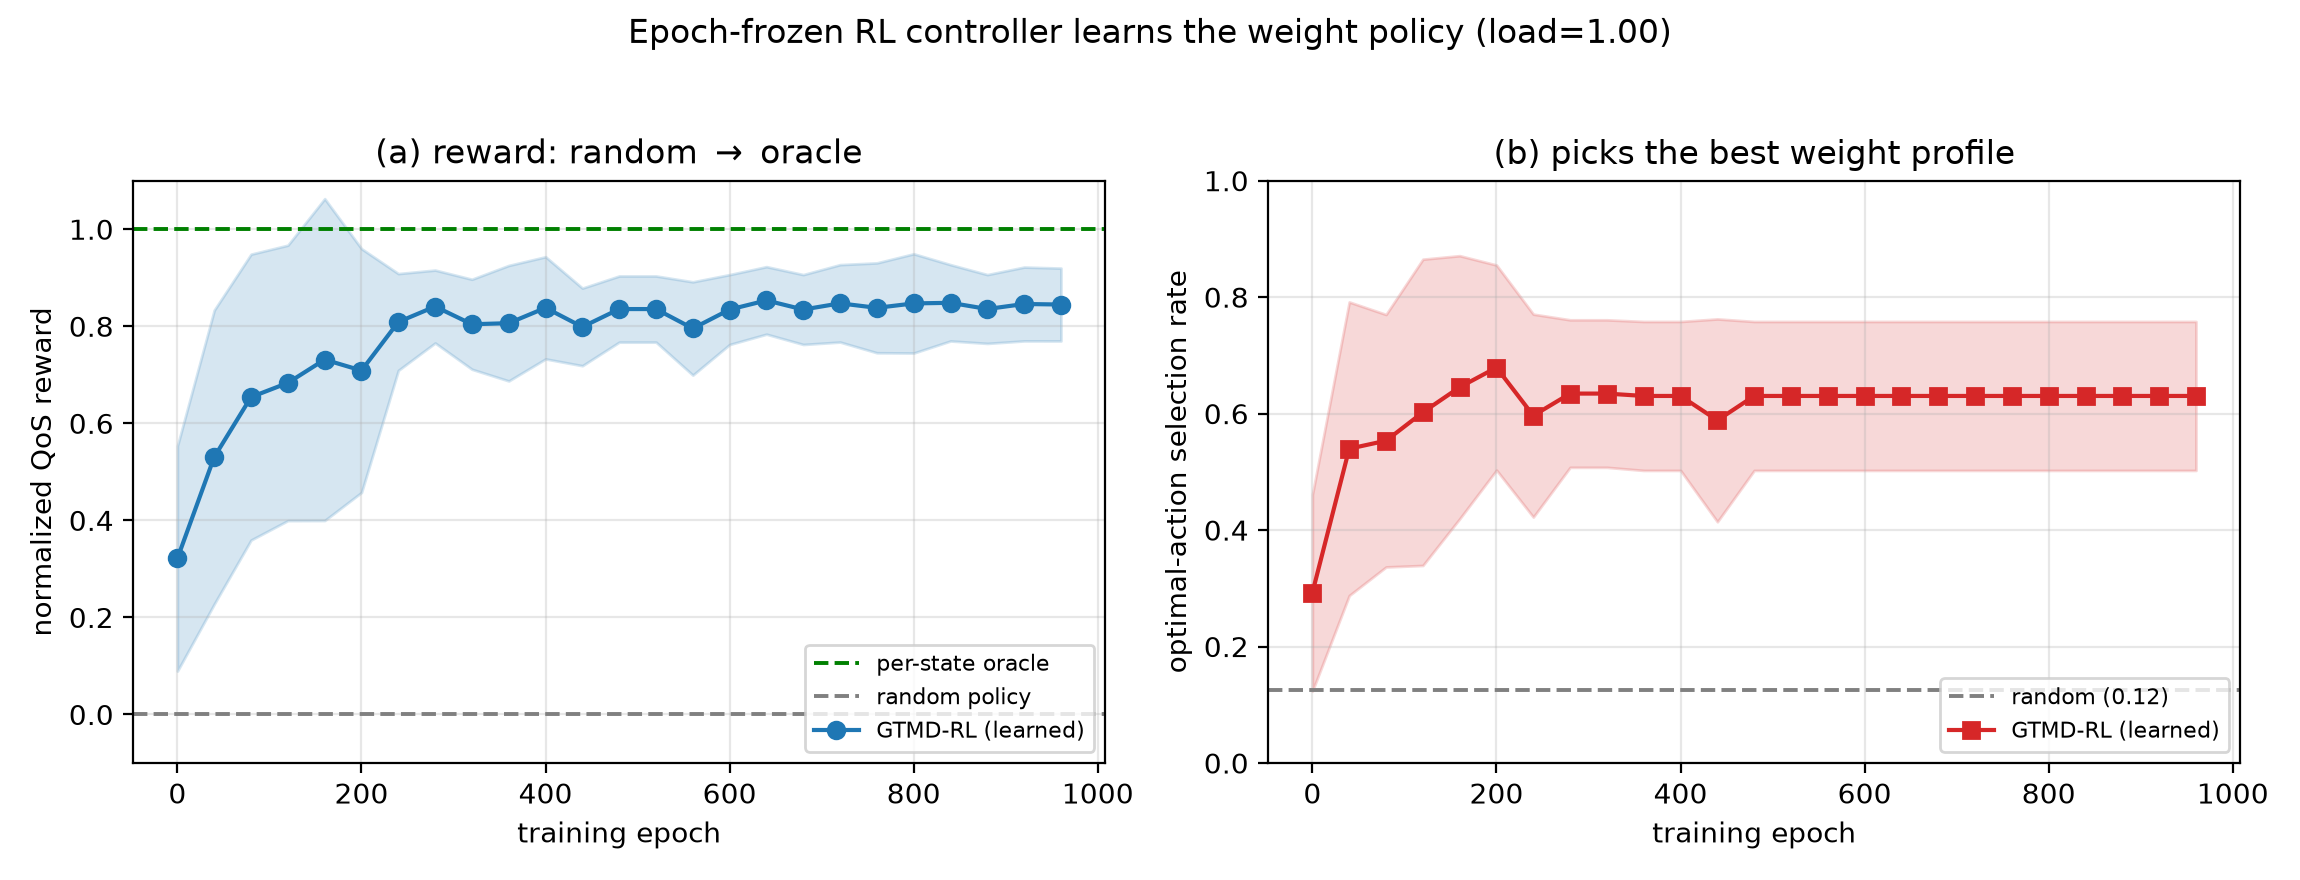
\includegraphics[width=0.99\columnwidth]{rl_learning_curve.png}
\caption{The epoch-frozen controller learns its weight policy. (a) normalized QoS reward rising from the random policy toward the per-context oracle; (b) rate of selecting the optimal weight profile rising from the $0.12$ random baseline. Mean $\pm$ std over $8$ seeds.}
\label{fig:learn}
\end{figure}

\textbf{Tabular vs.\ deep controllers.} To confirm the learning is not an artifact of the tabular representation and to test how the controller scales, we re-run the study with a larger action set (a $28$-point simplex lattice of weight profiles) and pit the tabular bandit against three deep controllers -- Double-DQN, PPO and A2C -- on the \emph{same} actions and reward. The deep agents replace the coarse two-bin context with the continuous demand belief (contention level, per-slice demand-to-floor stress, per-slice share); each epoch is a single-step episode, so they are contextual bandits, not sequential-MDP learners. All are scored by their greedy policy against the Monte-Carlo-true per-context action values ($0$ = random action, $1$ = per-context oracle), averaged over $3$ seeds and $3000$ epochs (Fig.~\ref{fig:deeprl}). PPO reaches the highest normalized reward ($0.62$), narrowly ahead of the exact tabular bandit ($0.59$) and DQN ($0.58$), which are statistically indistinguishable; A2C, the highest-variance method, lags at $0.21$. The deep policies exploit the continuous belief to resolve variation \emph{within} a tabular cell, which is why PPO/DQN match or edge the exact table despite a $28$-way action space; equally, the exact tabular bandit remains fully competitive at three slices, so the lightweight table is the sensible default and the deep controllers are the drop-in for larger slice/action spaces where a table no longer fits.

\begin{figure}[t]
\centering

\includegraphics[width=0.99\columnwidth]{deep_rl_comparison.png}
\caption{Tabular contextual bandit vs.\ deep controllers (DQN/PPO/A2C) on the same $28$-action simplex and priced-mechanism reward. (a) normalized reward and (b) optimal-action rate vs.\ training epoch (mean $\pm$ std, $3$ seeds); (c) converged normalized reward. PPO $\ge$ tabular $\approx$ DQN $\gg$ A2C.}
\label{fig:deeprl}
\end{figure}

\subsection{Truthfulness and robustness to misreporting}\label{sub:robust}
The frontier bounds the \emph{residual} slack; here we show operationally that the mechanism is strategy-proof and that truthfulness is what protects the system. We let the eMBB tenant scale its demand report by a persistent multiplier $m$ and compute its best response by grid search, everything on common random numbers so truthful and misreported runs differ only in the report. We compare five allocators on identical traffic: the floor-aware baselines (RR, max-CQI, PF); our priced DSIC mechanism (GTMD-RL); and -- the key ablation -- our \emph{same} allocator with the Myerson payment switched off (GTMD-noPay). The tenant's quasi-linear utility is its true-type valuation of the PRBs it can use, minus payments; a scheduler's manipulation gain is the best-response utility increase over truthful, and the collateral harm is the served-throughput the honest slices lose when the tenant games.

Fig.~\ref{fig:robust} is unambiguous. The utility curve $U(m)$ of GTMD-RL peaks \emph{exactly} at the truthful $m{=}1$ and falls for any misreport (panel a): truthful reporting is a dominant strategy, so the best response is $m^\star{=}1$ with $0\%$ gain, and the honest slices lose nothing. The identical allocator without the payment (GTMD-noPay) has a $U(m)$ that rises monotonically -- lying always pays -- yielding a $13.5\%$ best-response gain that starves the honest slices of $1.7$\,Mbps. This isolates the \emph{payment}, not the allocation rule, as the truthfulness lever. The demand-blind RR/max-CQI cannot be gamed ($0\%$ gain), but only because they discard the demand signal entirely; PF leaks a small $2\%$. The manipulation gain of the unpriced allocator climbs with contention (panel b), while GTMD-RL stays pinned at $0$ across all loads. The synthesis: on a demand-responsiveness (allocation sensitivity to the report) versus strategy-proofness ($100-$gain\%) plane, only GTMD-RL occupies the top-right corner -- it is the sole allocator that is both demand-responsive \emph{and} strategy-proof, because the payment prices manipulation away without throwing the demand signal out; the demand-blind baselines are strategy-proof only by discarding demand, and the unpriced allocator is responsive but gameable. Over the learning horizon this holds epoch by epoch: the truthful tenant's cumulative utility stays above any persistent misreport's and the gap grows monotonically (not shown, in the artifact).

\begin{figure*}[t]
\centering
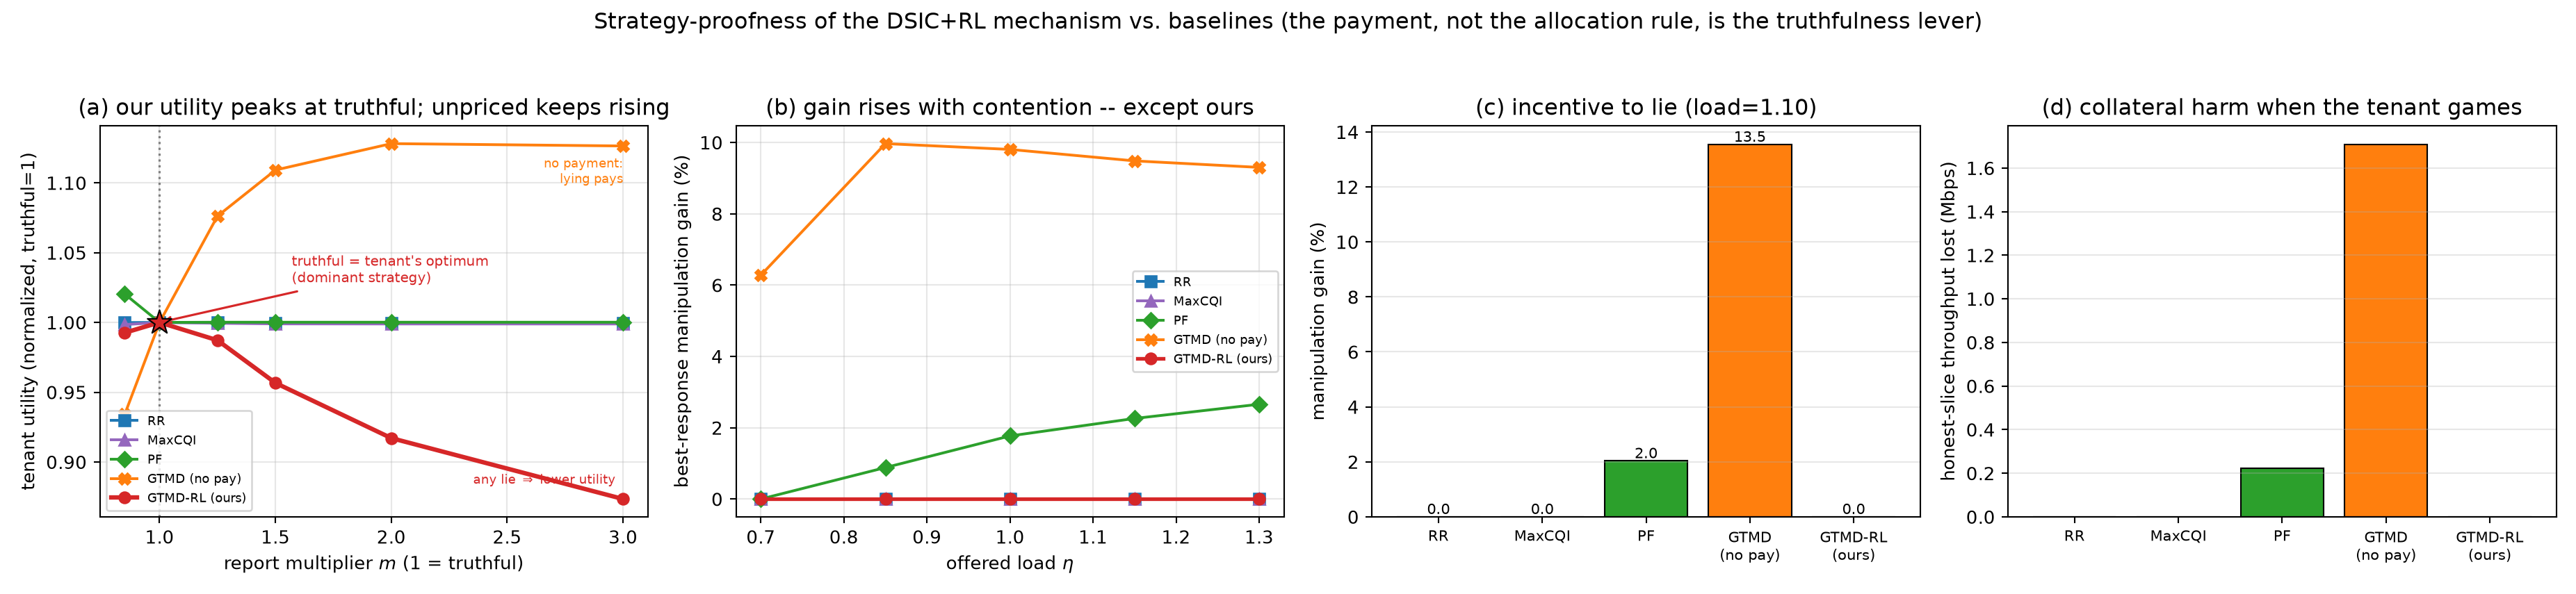
\includegraphics[width=0.98\textwidth]{robustness_dsic.png}
\caption{Strategy-proofness under strategic misreporting (best response, common random numbers). (a) Tenant utility vs.\ report multiplier: GTMD-RL peaks at the truthful $m{=}1$ (dominant strategy), while the same allocator without the payment (GTMD-noPay) keeps rising -- the payment is the truthfulness lever. (b) Best-response manipulation gain vs.\ load: $\sim\!0$ for GTMD-RL at every load, rising with contention for GTMD-noPay. (c) Manipulation gain and (d) throughput stolen from the honest slices, per scheduler, at $\load{=}1.1$.}
\label{fig:robust}
\end{figure*}

\subsection{Comparison with classical schedulers}\label{sub:compare}
We next ask whether the truthfulness guarantee costs performance. We compare GTMD-RL against round-robin (RR), max-CQI (best-rate), proportional-fair (PF) and their floor-aware variants (of which max-CQI$+$floors is the strongest baseline), all driven on identical arrival and channel realizations. Table~\ref{tab:compare} reports the slice-KPI panel at moderate ($\load{=}1.0$) and overloaded ($\load{=}1.3$) operating points; Fig.~\ref{fig:perslice} breaks the overloaded point out per slice.

\begin{table}[t]
\caption{GTMD-RL vs.\ classical schedulers on identical traffic ($\Slots{=}2400$). ``URLLC p95'' is the tail latency of the tight-SLA slice; ``floor'' is floor-satisfaction rate. Best in each block in \textbf{bold}. Only GTMD-RL is DSIC.}
\label{tab:compare}
\centering
\small
\setlength{\tabcolsep}{3pt}
\begin{tabular}{@{}l c c c c c@{}}
\toprule
Policy & Thr. & URLLC & $\pi$-wtd & waste & floor \\
       & (Mbps) & p95 (ms) & SLA & (PRB/slot) & sat. \\
\midrule
\multicolumn{6}{@{}l}{\textit{Load $\load=1.0$ (moderate)}}\\
Round-robin        & 16.73 & 1.90 & 0.236 & 1.35 & 0.99 \\
Max-CQI            & 16.73 & 2.06 & 0.298 & 1.37 & 0.99 \\
Proportional-fair  & 16.73 & 1.92 & 0.287 & 1.36 & 0.98 \\
Max-CQI$+$floors   & 16.73 & \textbf{0.70} & \textbf{0.091} & 8.92 & \textbf{1.00} \\
\textbf{GTMD-RL (ours)} & 16.73 & 1.46 & 0.151 & \textbf{2.18} & \textbf{1.00} \\
\midrule
\multicolumn{6}{@{}l}{\textit{Load $\load=1.3$ (overloaded)}}\\
Round-robin        & 23.17 & 3.73 & 1.278 & 0.91 & 0.94 \\
Max-CQI            & 23.17 & 4.65 & 0.987 & 1.05 & 0.91 \\
Proportional-fair  & 23.17 & 4.04 & 1.350 & 0.97 & 0.86 \\
Max-CQI$+$floors   & 23.17 & 3.93 & 1.001 & 4.71 & \textbf{1.00} \\
\textbf{GTMD-RL (ours)} & 23.17 & \textbf{2.02} & \textbf{0.711} & \textbf{1.57} & \textbf{1.00} \\
\bottomrule
\end{tabular}
\vspace{2pt}
{\footnotesize URLLC p95 is the tail latency of the tight-SLA ($2$\,ms) slice; $\pi$-wtd SLA $=\sum_i\pi_i\,$SLA$_i$ (Fig.~\ref{fig:perslice}); waste is idle reserved PRBs/slot. Among the floor-guaranteeing policies (\textbf{bold} = best of these) GTMD-RL is best on \emph{every} column under overload---URLLC tail, priority-weighted SLA, \emph{and} wasted PRBs---and best on waste at both loads; the demand-blind baselines undercut it only by violating floors ($0.86$--$0.99$). Only GTMD-RL is DSIC.}
\end{table}

\begin{figure}[t]
\centering
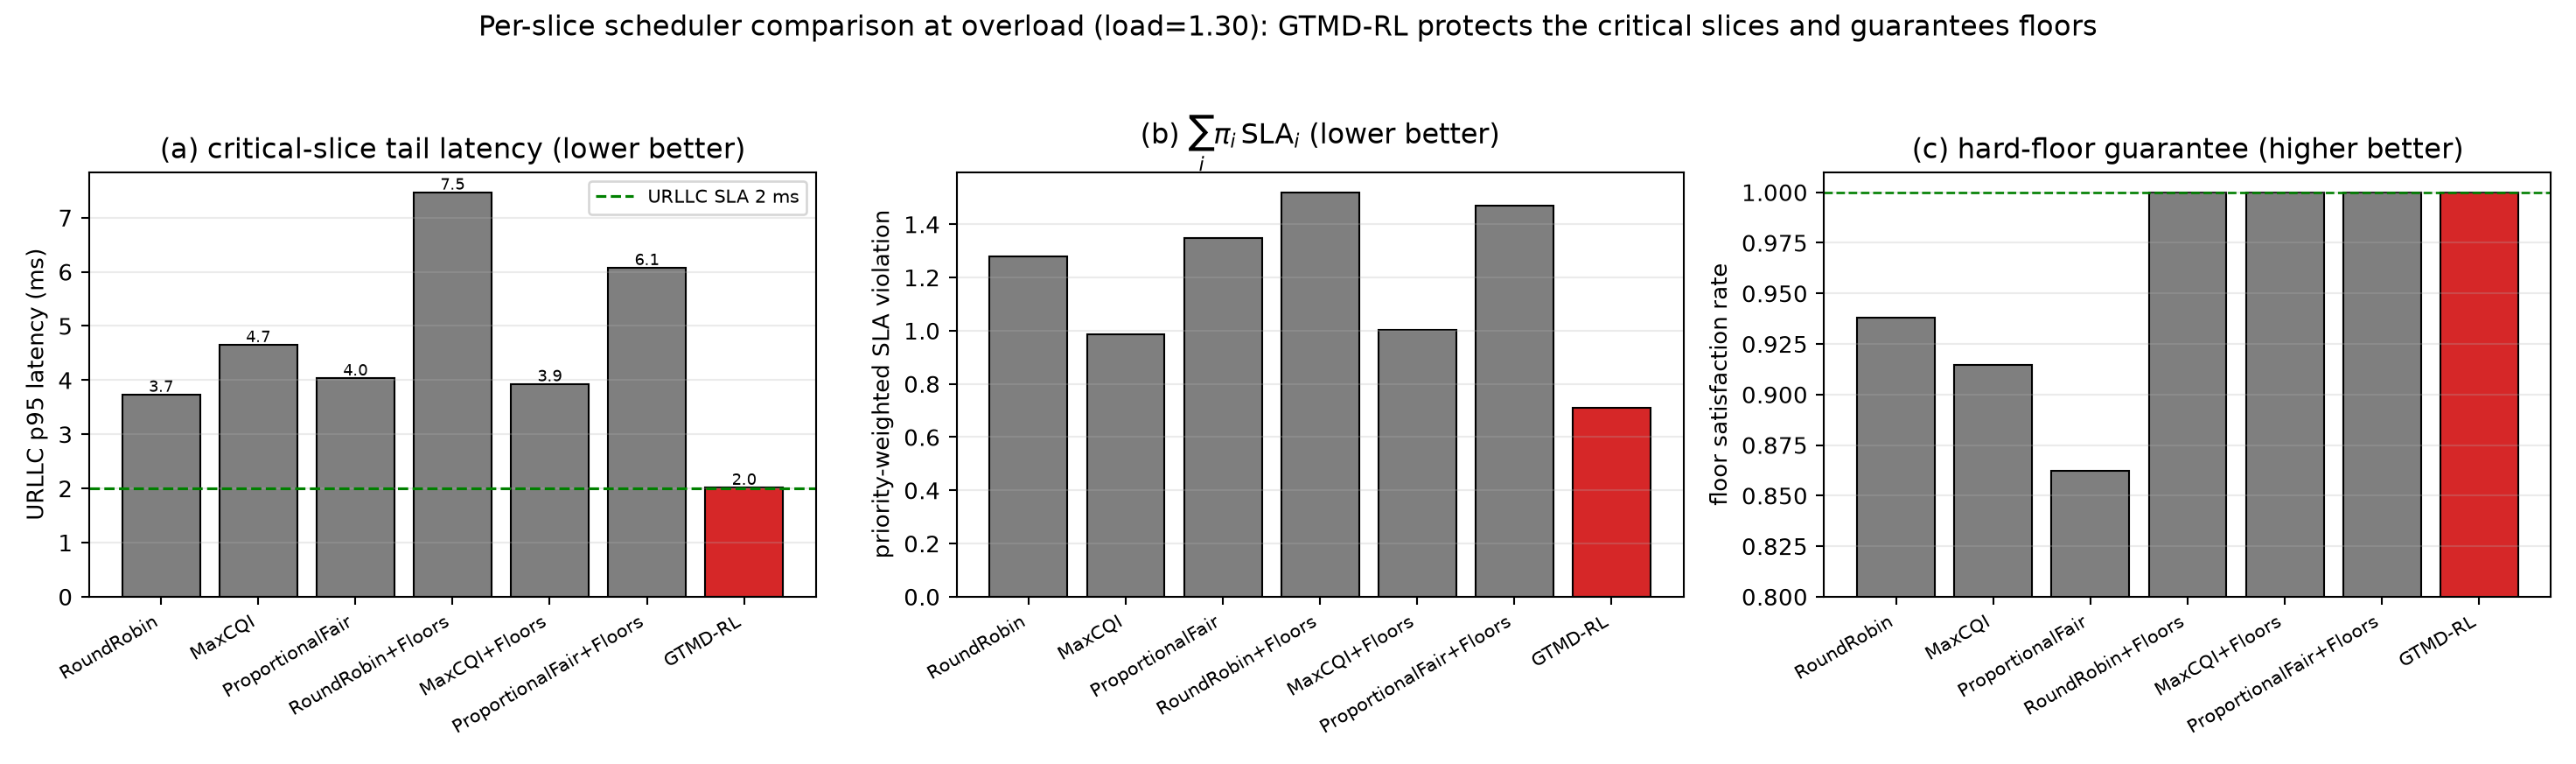
\includegraphics[width=0.99\columnwidth]{scheduler_perslice.png}
\caption{Per-slice view at overload ($\load{=}1.3$). The aggregate p95 is dominated by the delay-tolerant mMTC slice (20\,ms budget) and hides what matters: the deployed GTMD-RL scheduler---deadline- and channel-aware, with a small proactive burst headroom for the tight-SLA slice---delivers the \emph{lowest} URLLC tail latency (a), the \emph{best} priority-weighted SLA (b), and, uniquely among demand-aware policies, guarantees hard floors (c).}
\label{fig:perslice}
\end{figure}

Two findings stand out. First, \emph{truthfulness is free}: at every load GTMD-RL delivers the same aggregate throughput as the throughput-greedy max-CQI policy (arrival-limited below overload) and matches PF's fairness, so the incentive guarantee costs no efficiency. Second, \emph{it leads on the critical slice while staying spectrally efficient}: the deployed allocator orders the surplus by an M-LWDF-style metric (priority $\times$ deadline-urgency $\times$ channel gain), where the urgency is driven \emph{proactively} by the backlog a slice carries above its floor (scaled by $1/$SLA), and it reserves only a few PRBs of burst headroom for the tight-SLA slice. As a result, among the floor-guaranteeing policies GTMD-RL is best on \emph{every} QoS-and-efficiency column under overload at once: the lowest URLLC tail latency ($2.02$\,ms vs.\ $\ge3.9$\,ms), the best priority-weighted SLA ($0.711$), the lowest aggregate SLA, \emph{and} the fewest wasted PRBs ($1.57$ vs.\ $4.7$--$14.5$ for the floor-reserving baselines, which buy their low tails by parking idle spectrum). At moderate load all policies clear the URLLC budget comfortably, and the buffering baselines shave the tail below GTMD-RL only by wasting $4\times$ the spectrum. The one axis GTMD-RL does not lead is \emph{aggregate} p95 under overload: a priority scheduler deliberately makes the delay-tolerant mMTC slice wait, which the unweighted percentile penalises but the priority weighting rewards---the trade is intrinsic, and we verified that flattening it costs the URLLC and priority-weighted-SLA wins. GTMD-RL is thus the only policy that is simultaneously demand-aware, floor-guaranteeing, spectrally efficient, and DSIC; the single-lever ($\rhobind\!=\!1$) penalty appears in the frontier of Sec.~\ref{sub:frontier}, not here, since all deployed policies enforce floors.

\subsection{5G-LENA bridge validation}\label{sub:ns3}
Finally we close the loop on the real stack. We ran the Python controller as the
server and the compiled ns-3.46$+$5G-LENA scenario as the client over the TCP
bridge; the gNB received a per-slice PRB budget each epoch, ran the epoch on the NR
OFDMA PHY/MAC, and returned FlowMonitor KPIs that trained the RL policy. Table~\ref{tab:ns3}
reports the per-slice budget and the throughput and delay \emph{measured inside
ns-3}. The measured throughput tracks the PRB budget monotonically (eMBB, with the
largest budget, carries the most; mMTC, with the smallest, the least), confirming
that the socket-delivered allocation is faithfully enforced on the 3GPP MAC, and the
per-slice delays are in the few-millisecond range expected at this load. This is a
genuine closed control loop---learned policy in Python, radio stack in ns-3, plain
sockets between---not a co-simulation stub; the systematic sweeps of
Sections~\ref{sub:frontier}--\ref{sub:compare} use the faster controller-side
simulator that exports the identical mechanism.

\begin{table}[t]
\caption{Per-slice KPIs \emph{measured inside ns-3 5G-LENA} over the socket bridge (mean over epochs, $\load{\approx}1.0$). Throughput tracks the PRB budget, confirming faithful enforcement of the socket-delivered allocation.}
\label{tab:ns3}
\centering
\small
\setlength{\tabcolsep}{5pt}
\begin{tabular}{@{}l c c c@{}}
\toprule
Slice & PRB budget & Thr.\ (Mbps) & Delay (ms) \\
\midrule
URLLC & $19.6$ & $12.00$ & $3.66$ \\
eMBB  & $23.6$ & $13.26$ & $3.77$ \\
mMTC  & $6.8$  & $2.26$  & $4.05$ \\
\bottomrule
\end{tabular}
\end{table}

\textbf{Overhead.} The control-plane message is a single newline-delimited JSON line
per epoch carrying $O(\Ntn)$ scalars (budget, weights, reports, capacities), a few
hundred bytes; at the epoch cadence ($\Ep=30$--$240$ slots, i.e.\ tens to hundreds of
ms) this is negligible relative to E2 signalling, and it matches the near-RT-RIC
$10$\,ms--$1$\,s control-loop budget. The inner allocator is $O(\Ntn\log\Ntn)$ per slot
(a sort plus a greedy fill), and the Myerson payment adds one $O(\Ntn\,G)$ pass over a
$G$-point report grid per epoch; both are dominated by the PHY/MAC cost.

\section{Limitations}\label{sec:limits}
The private type is scalar and single-crossing; a Bayesian estimator of the demand-generating distribution and a $(\min,+)$ service-curve generalization of the valuation are natural extensions deferred to a journal version. The lower bound in Theorem~\ref{thm:frontier} is stated for the epoch-frozen monotone-allocator class rather than universally. The rate-cap PRB enforcement in the bridge is a faithful but coarse realization of a MAC-level per-slice budget; the scheduler-subclass variant is the exact realization. Validation is in a 3GPP-compliant simulator rather than a hardware testbed.

\section{Conclusion}\label{sec:concl}
We showed that learning a truthful PRB allocator under hard service floors faces an incentive--learning tradeoff governed by two parameters, the epoch length and the service-floor binding frequency, the latter being an exogenous, measurable quantity. The resulting frontier is strictly better than the known single-lever barrier in the underloaded regime O-RAN targets. We instantiate the mechanism as an epoch-frozen DSIC-RL allocator, couple it to ns-3 5G-LENA over a plain socket, and show empirically that the incentive slack vanishes exactly where floors stop binding, that the binding frequency is set by load and not the learning horizon, and that, under overload, the truthful learned allocator is best among floor-guaranteeing schedulers on URLLC tail latency, priority-weighted SLA, aggregate SLA and spectral efficiency simultaneously, while uniquely guaranteeing floors. A strategic-reporting study confirms the mechanism is dominant-strategy truthful in practice---the tenant's best response is exactly truthful, whereas the same allocator with the payment removed is gamed for a double-digit utility gain that starves the honest slices---identifying the payment as the lever that renders a demand-responsive learner strategy-proof.

\section*{Acknowledgment}
The authors thank colleagues at the LAN Lab, IIT Kharagpur.

\appendices

\section{Full proof of Theorem~\ref{thm:imposs}}\label{app:imposs}
Let $u_i^{>k}(\hat\type_{i,k})$ denote tenant $i$'s cumulative utility over epochs $>k$ as a function of its epoch-$k$ report, with all else fixed and others truthful. Differentiating through the weight map,
\[
\frac{d u_i^{>k}}{d\hat\type_{i,k}}=\sum_{t>kL}\Big\langle\nabla_{\wt}\,u_{i,t},\ \frac{\partial\wt}{\partial\hat\type_{i,k}}\Big\rangle .
\]
Write the per-epoch allocation as the solution of the constrained program $\max_{\alloc\in\allocsp}\sum_j\wt_j\val_j(\alloc_j;\hat\type_j)$ s.t. $\alloc_{j}\ge\flo_j$ on constrained slots. The KKT conditions give, at slot $t$, $\wt_i\partial_{\alloc_i}\val_i=\lambda_t-\mu_{i,t}$, with $\lambda_t$ the PRB-budget multiplier and $\mu_{i,t}\ge0$ the floor multiplier, $\mu_{i,t}>0$ only when the floor binds. The gradient $\nabla_{\wt}u_{i,t}$ splits into a term proportional to $(\lambda_t-\wt_i\partial_{\alloc_i}\val_i)$, which the learner's welfare ascent already drives to zero in expectation at an interior optimum, and a residual proportional to $\mu_{i,t}$. On non-binding slots $\mu_{i,t}=0$ and, by Assumption~\ref{ass:mono} (continuity of $g$ in $\wt$), the remaining term is first-order zero by the envelope theorem. On binding slots the residual $\mu_{i,t}\,\partial\wt/\partial\hat\type_{i,k}$ survives. Taking expectations and summing yields \eqref{eq:slacklocal}; the supports coincide with $\{t:\bindind_t=1\}$, so $\rhobind=0\Rightarrow\Slack_i=0$. Non-triviality of $\partial\wt/\partial\hat\type_{i,k}$ and $\rhobind>0$ make the residual generically nonzero, establishing the failure of exact dynamic IC. \hfill$\blacksquare$

\section{Full proof of Theorem~\ref{thm:frontier}}\label{app:frontier}
\emph{Regret.} Index epochs $k=1,\dots,\Neps$. Define the per-epoch loss $\ell_k(\wt)=-\sum_{t\in\text{epoch }k}r_t(\wt)$, with per-slot reward $r_t\in[0,1]$, so $\ell_k$ has range $[0,\Ep]$ and $O(\Ep)$-bounded subgradients over the bounded weight domain. Online gradient descent over $\Neps$ rounds attains $\sum_k\ell_k(\wt_k)-\min_{\wt}\sum_k\ell_k(\wt)=O(\Ep\sqrt{\Neps})$. Substituting $\Neps=\Slots/\Ep$ gives $\Reg(\Slots)=\Otil(\Ep\sqrt{\Slots/\Ep})=\Otil(\sqrt{\Ep\Slots})$.

\emph{Slack.} Fix tenant $i$. By Appendix~\ref{app:imposs} the per-epoch manipulation gain is $\sum_{t\in\text{epoch }k+1}\bindind_t\,\mu_{i,t}\,\langle\partial\wt/\partial\hat\type_{i,k},\cdot\rangle$. Assumption~\ref{ass:infl} bounds $\lVert\partial\wt/\partial\hat\type_{i,k}\rVert=O(1/\Ep)$; the expected number of binding slots in an epoch is $\rhobind\Ep$ and $\mu_{i,t}$ is uniformly bounded, so the per-epoch gain is $O(\rhobind\Ep\cdot1/\Ep)=O(\rhobind)$. Summing over $\Neps=\Slots/\Ep$ epochs gives $\Slack(\Slots)=O(\rhobind\Slots/\Ep)$.

\emph{Balance and optimum.} Minimizing $\sqrt{\Ep\Slots}+\rhobind\Slots/\Ep$ over $\Ep$, the first-order condition $\tfrac12\sqrt{\Slots/\Ep}=\rhobind\Slots/\Ep^{2}$ gives $\Ep^{3/2}=\Theta(\rhobind\Slots^{1/2})$, hence $\Ep^\star=\Theta(\rhobind^{2/3}\Slots^{1/3})$ and objective value $\Otil(\rhobind^{1/3}\Slots^{2/3})$.

\emph{Lower bound (class-restricted).} Within the epoch-frozen monotone-allocator class, an algorithm that updates $\Neps$ times incurs switching structure to which the $\Omega(\Slots^{2/3})$ bandit-switching lower bound of~\cite{ref:dekel} applies when every slot can bind ($\rhobind=1$); reducing the binding mass to a $\rhobind$-fraction scales the manipulable signal by $\rhobind$, matching the upper bound up to logarithmic factors. \hfill$\blacksquare$

\section{Full proof of Lemma~\ref{lem:invariance}}\label{app:invariance}
Within epoch $k$ the weight $\wt_k$ is constant, so the slot-indexed allocation process $\{\alloc_t\}_{t\in\text{epoch }k}$ is a deterministic measurable map of the stationary ergodic arrival process (Assumption~\ref{ass:stat}). The binding indicator $\bindind_t=\ind[\text{floor active and limiting}]$ is a fixed measurable functional of $(\alloc_t,\text{arrivals}_t)$, hence itself stationary ergodic within the epoch. By Birkhoff's ergodic theorem the within-epoch average $\tfrac1\Ep\sum_{t\in\text{epoch }k}\bindind_t\to\E[\bindind]=\rhobind^\star(\load)$ almost surely as $\Ep\to\infty$, where $\rhobind^\star(\load)$ is the stationary binding probability fixed by the load factor and floor levels and independent of $\Ep$. The single weight change at the epoch boundary perturbs the process over an $O(1)$-length transient, contributing an $O(1/\Ep)$ correction to the epoch average. Averaging over epochs preserves the bound, giving $\rhobind(\Ep,\load)=\rhobind^\star(\load)+O(1/\Ep)$. \hfill$\blacksquare$

\begin{thebibliography}{00}
\bibitem{ref:oran} M.~Polese \emph{et al.}, ``Understanding O-RAN: Architecture, interfaces, algorithms, security, and research challenges,'' \emph{IEEE Commun. Surveys Tuts.}, vol.~25, no.~2, pp.~1376--1411, 2023.
\bibitem{ref:coloran} L.~Bonati \emph{et al.}, ``ColO-RAN: Developing machine learning-based xApps for open RAN closed-loop control on programmable experimental platforms,'' \emph{IEEE Trans. Mobile Comput.}, vol.~22, no.~10, 2023.
\bibitem{ref:slicing} D.~Bega \emph{et al.}, ``Network slicing meets artificial intelligence: An AI-based framework for slice management,'' \emph{IEEE Commun. Mag.}, vol.~58, no.~6, pp.~32--38, 2020.
\bibitem{ref:myerson} R.~B. Myerson, ``Optimal auction design,'' \emph{Math. Oper. Res.}, vol.~6, no.~1, pp.~58--73, 1981.
\bibitem{ref:huh} J.~Huh and K.~Kandasamy, ``Nash incentive-compatible online mechanism learning via weakly differentially private online learning,'' in \emph{Proc. ICML}, 2024.
\bibitem{ref:dai} Y.~Dai, N.~Golrezaei, and P.~Jaillet, ``Incentive-aware dynamic resource allocation under long-term cost constraints,'' arXiv:2507.09473, 2025.
\bibitem{ref:dekel} O.~Dekel, J.~Ding, T.~Koren, and Y.~Peres, ``Bandits with switching costs: $T^{2/3}$ regret,'' in \emph{Proc. STOC}, 2014.
\bibitem{ref:bergemann} D.~Bergemann and J.~V\"alim\"aki, ``The dynamic pivot mechanism,'' \emph{Econometrica}, vol.~78, no.~2, pp.~771--789, 2010.
\bibitem{ref:kakade} S.~Kakade, I.~Lobel, and H.~Nazerzadeh, ``Optimal dynamic mechanism design and the virtual-pivot mechanism,'' \emph{Oper. Res.}, vol.~61, no.~4, pp.~837--854, 2013.
\bibitem{ref:slicinggames} P.~Caballero \emph{et al.}, ``Network slicing games: Enabling customization in multi-tenant mobile networks,'' \emph{IEEE/ACM Trans. Netw.}, vol.~27, no.~2, pp.~662--675, 2019.
\bibitem{ref:pf} A.~Jalali, R.~Padovani, and R.~Pankaj, ``Data throughput of CDMA-HDR: A high efficiency-high data rate personal communication wireless system,'' in \emph{Proc. IEEE VTC}, 2000.
\bibitem{ref:5glena} N.~Patriciello, S.~Lag\'en, B.~Bojovi\'c, and L.~Giupponi, ``An E2E simulator for 5G NR networks,'' \emph{Simul. Model. Pract. Theory}, vol.~96, 2019.
\bibitem{ref:ns3ai} H.~Yin \emph{et al.}, ``ns3-ai: Fostering artificial intelligence algorithms for networking research,'' in \emph{Proc. ACM WNS3}, 2020.
\bibitem{ref:sb3} A.~Raffin \emph{et al.}, ``Stable-Baselines3: Reliable reinforcement learning implementations,'' \emph{J. Mach. Learn. Res.}, vol.~22, no.~268, pp.~1--8, 2021.
\bibitem{ref:netcalc} J.-Y. Le Boudec and P.~Thiran, \emph{Network Calculus}. Springer LNCS 2050, 2001.
\end{thebibliography}

\end{document}
